\documentclass[a4paper,boxed,11pt]{caspset}




% set 1-inch margins in the document
%\usepackage[left=1in,right=1in,top=1.2in,bottom=1in]{geometry}
\usepackage[left=1in,right=1in,top=1.2in,bottom=1in]{geometry}
\usepackage{lastpage}
\usepackage{geometry}
% include this if you want to import graphics files with /includegraphics
\usepackage{multicol} 
\usepackage{capt-of}%%To get the caption
\usepackage{graphicx}
\usepackage{lscape}
\usepackage{amsmath,amsfonts,amsthm,amssymb}
\usepackage{mathtools}
\usepackage[usenames,dvipsnames]{color}
\usepackage{hyperref}
\usepackage{fancyhdr}
\usepackage{lastpage}
\usepackage{extramarks}
\usepackage{chngpage}
\usepackage{soul}
\usepackage{ifthen}
\usepackage{listings}
\usepackage{courier}
\usepackage{multimedia}
\usepackage[toc,page,title,titletoc,header]{appendix}
\usepackage{color, soul}
\usepackage{array}
\usepackage{attachfile2}
\usepackage{tikz}
\usepackage{pgfplots}
%%%%%%%%%%%%%%%%%%%%%%%%%%%%%%%%%%%%%%%%%%%%%%%%%%%%%%
\usepackage{xeCJK}
%\usepackage{fontspec}
\setCJKmainfont[BoldFont=simhei.ttf]{simsun.ttf}
%\setCJKsansfont{simhei.ttf}
%\setCJKmonofont{simfang.ttf}

%\setCJKmainfont{Adobe Song Std}
%\setCJKmainfont[BoldFont=Adobe Heiti Std]{Adobe Song Std}
%%%%%%%%%%%%%%%%%%%%%%%%%%%%%%%%%%%%%%%%%%%%%%%%%%%%%%


\graphicspath{{figures/}}

\setulcolor{red}

\setlength{\marginparwidth}{1in}

\newcommand{\hmwkTitle}{高等计算流体力学}
\newcommand{\hmwkSubTitle}{高等计算流体力学课程家庭作业题(A2)}
\newcommand{\hmwkDueDate}{\today}
\newcommand{\hmwkClass}{物理学院}
\newcommand{\hmwkClassTime}{Tue/Thu.{~}09:50}
\newcommand{\hmwkClassInstructor}{张德良}
\newcommand{\hmwkAuthorName}{周吕文}

\hypersetup{pdfauthor={\hmwkAuthorName}, 
            pdftitle={不可压缩二维N-S方程的SIMPLE解法}, 
            pdfsubject={\hmwkTitle, \hmwkClassInstructor},
            pdfkeywords={高等计算流体, 不可压缩二维N-S方程, SIMPLE解法},
            pdfproducer={XeLateX with hyperref},
            pdfcreator={Xelatex}}


%% Setup the header and footer
\pagestyle{fancy}                                                       %
\lhead{\hmwkAuthorName}                                                 %
\chead{\hmwkClass\ (\hmwkClassInstructor): \hmwkTitle}  %
\rhead{第\ \thepage\ 页,{~} 共\ \protect\pageref{LastPage} 页}          %                                %
\definecolor{DarkGreen}{rgb}{0.0,0.45,0.0}

%%%%%%%%%%%%%%%%%%%%%%%%%%%%%%%%%%%%%%%%%%%%%%%%%%%%%%%%%%%%%



\makeatletter
\newcommand{\rmnum}[1]{\romannumeral #1}
\newcommand{\Rmnum}[1]{\expandafter\@slowromancap\romannumeral #1@}
\makeatother

\renewcommand\refname{\bf\large 参考文献}
\renewcommand\contentsname{\bf 目 \ \ \ 录}
\renewcommand\figurename{\bf 图}
\renewcommand\tablename{\bf 表}
\renewcommand{\appendixtocname}{附录}
\renewcommand{\appendixpagename}{附录}
\renewcommand\listfigurename{图目录}

\name{周吕文{~}201128000718065}
\class{物理学院{~}20110308班}
\assignment{计算报告}
\duedate{4/15/2012}

\newcommand\invisiblesection[1]{%
  \refstepcounter{section}%
  \addcontentsline{toc}{section}{\protect\numberline{\thesection}#1}%
  \sectionmark{#1}}

\newcommand\invisiblesubsection[1]{%
  \refstepcounter{subsection}%
  \addcontentsline{toc}{subsection}{\protect\numberline{\thesubsection}#1}%
  \subsectionmark{#1}}


\newcommand{\matlabscript}[2]
{\definecolor{MyDarkGreen}{rgb}{0.0,0.3,0.0}
\definecolor{hellgelb}{rgb}{0.96,0.96,0.96}
\definecolor{DarkPurple}{rgb}{0.6,0,0.4}
    \lstset{%
       language=Matlab,                        % Use MATLAB
        frame=single,                           % Single frame around code
        basicstyle=\footnotesize\ttfamily,    
        keywordstyle=[1]\color{blue}, 
        keywordstyle=[2]\color{DarkPurple}, 
        keywordstyle=[3]\color{blue}\underbar, 
        identifierstyle=,  
        commentstyle=\color{MyDarkGreen}\footnotesize,
        stringstyle=\color{DarkPurple}, 
        showstringspaces=false,            
        tabsize=5,     
        morekeywords={xlim,ylim,var,alpha,factorial,poissrnd,normpdf,normcdf},
        morekeywords=[2]{on, off, interp},
        morecomment=[l][\color{blue}]{...},    
     columns=fixed,
     tabsize=4,%
     numbers=left,                           % Line numbers on left
     firstnumber=1,                          % Line numbers start with line 1
     numberstyle=\tiny\color{Blue},          % Line numbers are blue
     stepnumber=5,                            % Line numbers go in steps of 5
framexleftmargin=1mm, framextopmargin=1mm, frame=shadowbox
    }
\lstinputlisting[caption=#2]{#1.m}}
%%%%%%%%%%%%%%%%%%%%%%%%%%%%%%%%%%%%%%%%%%%%%%%%%%%%%%%%%%%%%
% This gives syntax highlighting in the python environment
\newcommand{\fortranscript}[2]
{
\definecolor{gray}{gray}{0.4}
\definecolor{key}{rgb}{0.3,1,0.3}
\lstset{
language=[90]fortran,
basicstyle=\ttfamily,
%otherkeywords={1, 2, 3, 4, 5, 6, 7, 8 ,9 , 0, -, =, +, [, ], (, ), \{, \}, :, *, !},
keywordstyle=\color{blue},
stringstyle=\color{red},
showstringspaces=false,
        numbers=left,                           % Line numbers on left
        firstnumber=1,                          % Line numbers start with line 1
        numberstyle=\tiny\color{Blue},          % Line numbers are blue
        stepnumber=5,                            % Line numbers go in steps of 5
commentstyle=\color{gray},%\slshape,
framexleftmargin=1mm, framextopmargin=1mm, frame=shadowbox
}
\lstinputlisting[caption=#2]{#1.f90}
}

\begin{document}

\problemlist{\LARGE 不可压缩二维N-S方程的SIMPLE解法}

\section{引言}
SIMPLE算法全称是``Semi-Implicit Method for Pressure-Linked Equations'',
意思是求解压力耦合的质量/动量/能量传递方程的半隐式方法. SIMPLE 算法自1972年由
D.B.Spalding 和 S.V.Patankar提出以来在世界各国计算流体力学及计算传热学界得到了广泛的应用,
它实际上已经成为许多工程流动, 传热以及反应体系的数值模拟的最重要的方法. 许多商业CFD软件, 如cfx 与fluent, 其核心也都基于SIMPLE
算法.

SIMPLE算法适合求解不可压流场的数值问题, 也可用于求解可压流动. 它的核心是采用``猜测-修正''的过程. 基本思想: 对于给定的压力场(它可以是假定值或是上一次迭代计算所得到的结果),
求解离散形式的动量方程, 得出速度场. 因为压力场是假定的或不精确的, 这样得到的速度场一般不满足连续方程, 因此, 必须对给定的压力场加以修正.
修正的原则是: 与修正后的压力场相对应的速度场能满足这一迭代层次上的连续方程离散形式. 据此原则, 我们把由动量方程的离散形式所规定的压力与速度的关系代入连续方程的离散形式,
从而得到压力修正方程, 由压力修正方程得出压力修正值. 接着, 根据修正后的压力场, 求得新的速度场. 然后检查速度场是否收敛. 若不收敛,
用修正后的压力值作为给定的压力场, 开始下一层次的计算, 直至收敛为止.
\section{不可压缩二维N-S方程}

对于二维的不可压缩问题, 其N-S方程描述为
\begin{align}
u_{t}+p_{x} & =-\big(uu\big)_{x}-\big(uv\big)_{y}+\frac{1}{Re}\big(u_{xx}+u_{yy}\big)\label{momentumU}\\
v_{t}+p_{y} & =-\big(uv\big)_{x}-\big(vv\big)_{y}+\frac{1}{Re}\big(v_{xx}+v_{yy}\big)\label{momentumV}\\
u_{x}+v_{y} & =0
\end{align}
其中$u$, $v$分别是$x$和$y$方向的速度, $p$为压强, $Re$是雷诺数.


\section{SIMPLE算法}

根据SIMPLE算法, 首先本文需要设定一个初始压力场$(P^{*})^{n}$, 以及初始速度场$(U^{*})^{n}$和$(U^{*})^{n}$,
然后根据动量方程求出$(U^{*})^{n+1}$和$(U^{*})^{n+1}$, 再通过解压力校正方程
\[
\nabla^{2}p'=\frac{1}{\Delta t}(\nabla\cdot V)
\]
来求得压力校正值$p'$, 将猜测值$p^{*}$与校正值$p'$合成. 然后得到修正后的压力场和速度场. SIMPLE算法的步骤如图\ref{steps}所示.
\newpage
\begin{figure}[!htb]
\centering
%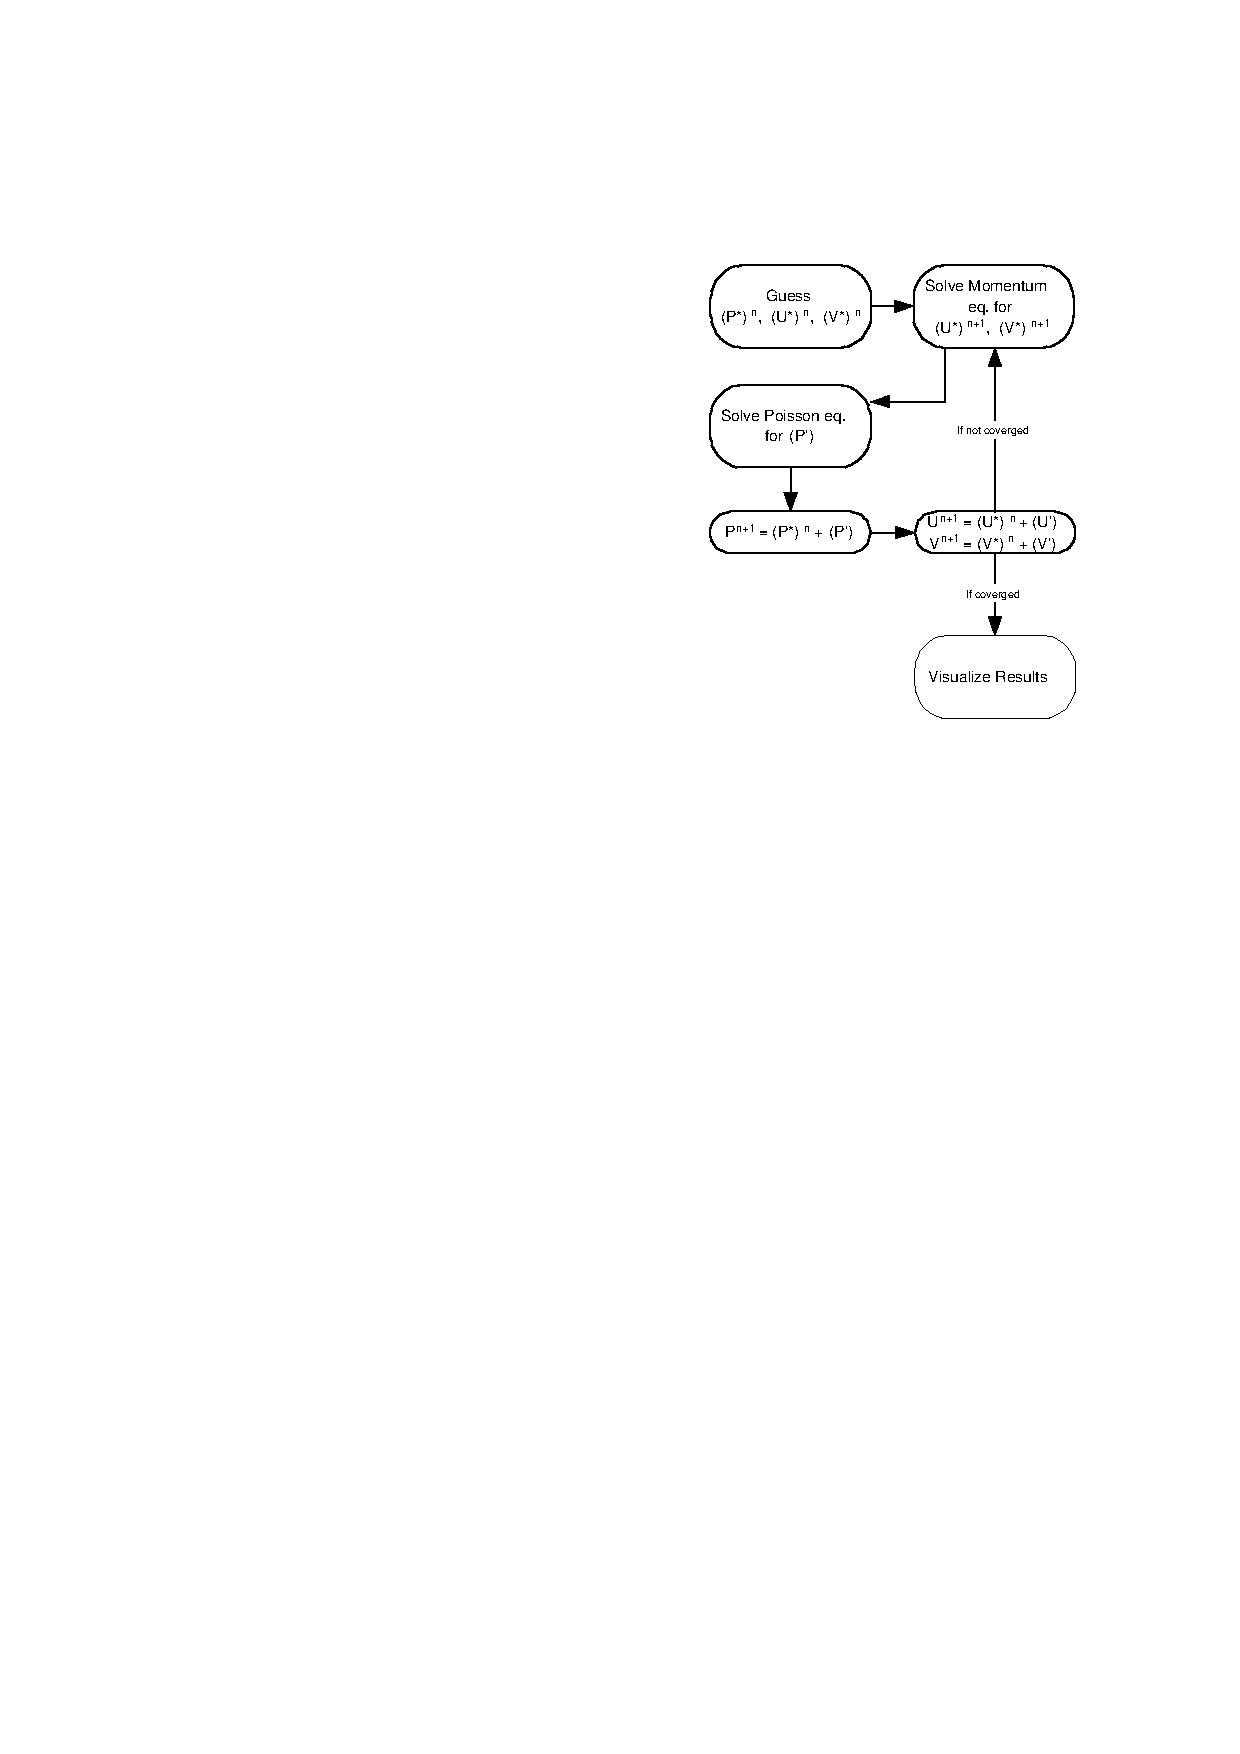
\includegraphics[width=0.45\textwidth]{./figures/steps.pdf}
\usetikzlibrary{shapes,arrows}


% Define block styles
\tikzstyle{decision} = [diamond, draw, fill=blue!20, 
    text width=5em, text badly centered, node distance=3cm, inner sep=0pt]
\tikzstyle{block} = [rectangle, draw, fill=blue!20, 
    text width=15em, text centered, rounded corners, minimum height=4em]
\tikzstyle{line} = [draw, -latex']
\tikzstyle{cloud} = [draw, ellipse,fill=red!20, node distance=4cm,
    minimum height=2em]
    
\begin{tikzpicture}[node distance = 2cm, auto]
    % Place nodes
    \node [block] (init) {开始};
    \node[block, below of=init](initvalue){初始化各参数的值}; 
    \node[block, below of=initvalue](cfl){根据CFL条件计算时间步差$\Delta t$ \\Function: timestep}; 
    %\node [cloud, left of=init] (expert) {expert};
    %\node [cloud, right of=init] (system) {system};
    \node [block, below of=cfl] (identify) {计算人工黏性项\\Function: artificial\_visc};
    \node [block, below of=identify] (evaluate) {按照蛙跳格式计算$u_j^{n+1}$\\Subroutine: leapfrog };
    \node [block, below of=evaluate] (boundary) {根据反射边界条件修正$u_j^{n+1}$\\Subroutine: boundary };
    \node [cloud, left of=evaluate, node distance=4.5cm] (update) {$t=t+\Delta t$};
    \node [decision, below of=boundary,node distance=2.5cm] (decide) {$t>t_{\textrm{end}}$?};
    \node [block, below of=decide, node distance=2.75cm] (stop) {结束并输出结果\\
Subrountine: output };
    % Draw edges
    \path [line] (init) -- (initvalue);
    \path [line] (initvalue)--(cfl);
    \path [line] (cfl)--(identify);
    \path [line] (identify) -- (evaluate);
    \path [line] (evaluate) -- (boundary);
    \path [line] (boundary)--(decide);
    \path [line] (decide) -| node [near start] {yes} (update);
    \path [line] (update) |- (cfl);
    \path [line] (decide) -- node {no}(stop);
    %\path [line,dashed] (expert) -- (init);
   % \path [line,dashed] (system) -- (init);
   % \path [line,dashed] (system) |- (evaluate);
\end{tikzpicture}

\caption{\label{steps}SIMPLE算法的步骤}
\end{figure}

\subsection{交错网格}
为了对不可压缩二维N-S方程离散差分, 本文选则如图\ref{Stagger}所示的矩形交错网格. 把速度分量和压力分量分别设置在三套不同的网格单元上. 其中压力设置在主控制单元的中心. 相应的水平方向速度$u$设置在主控制单元的左右边界上, 相应的竖直方向速度$v$设置在主控制单元的上下边界上.

\begin{figure}[!htb]
\centering
%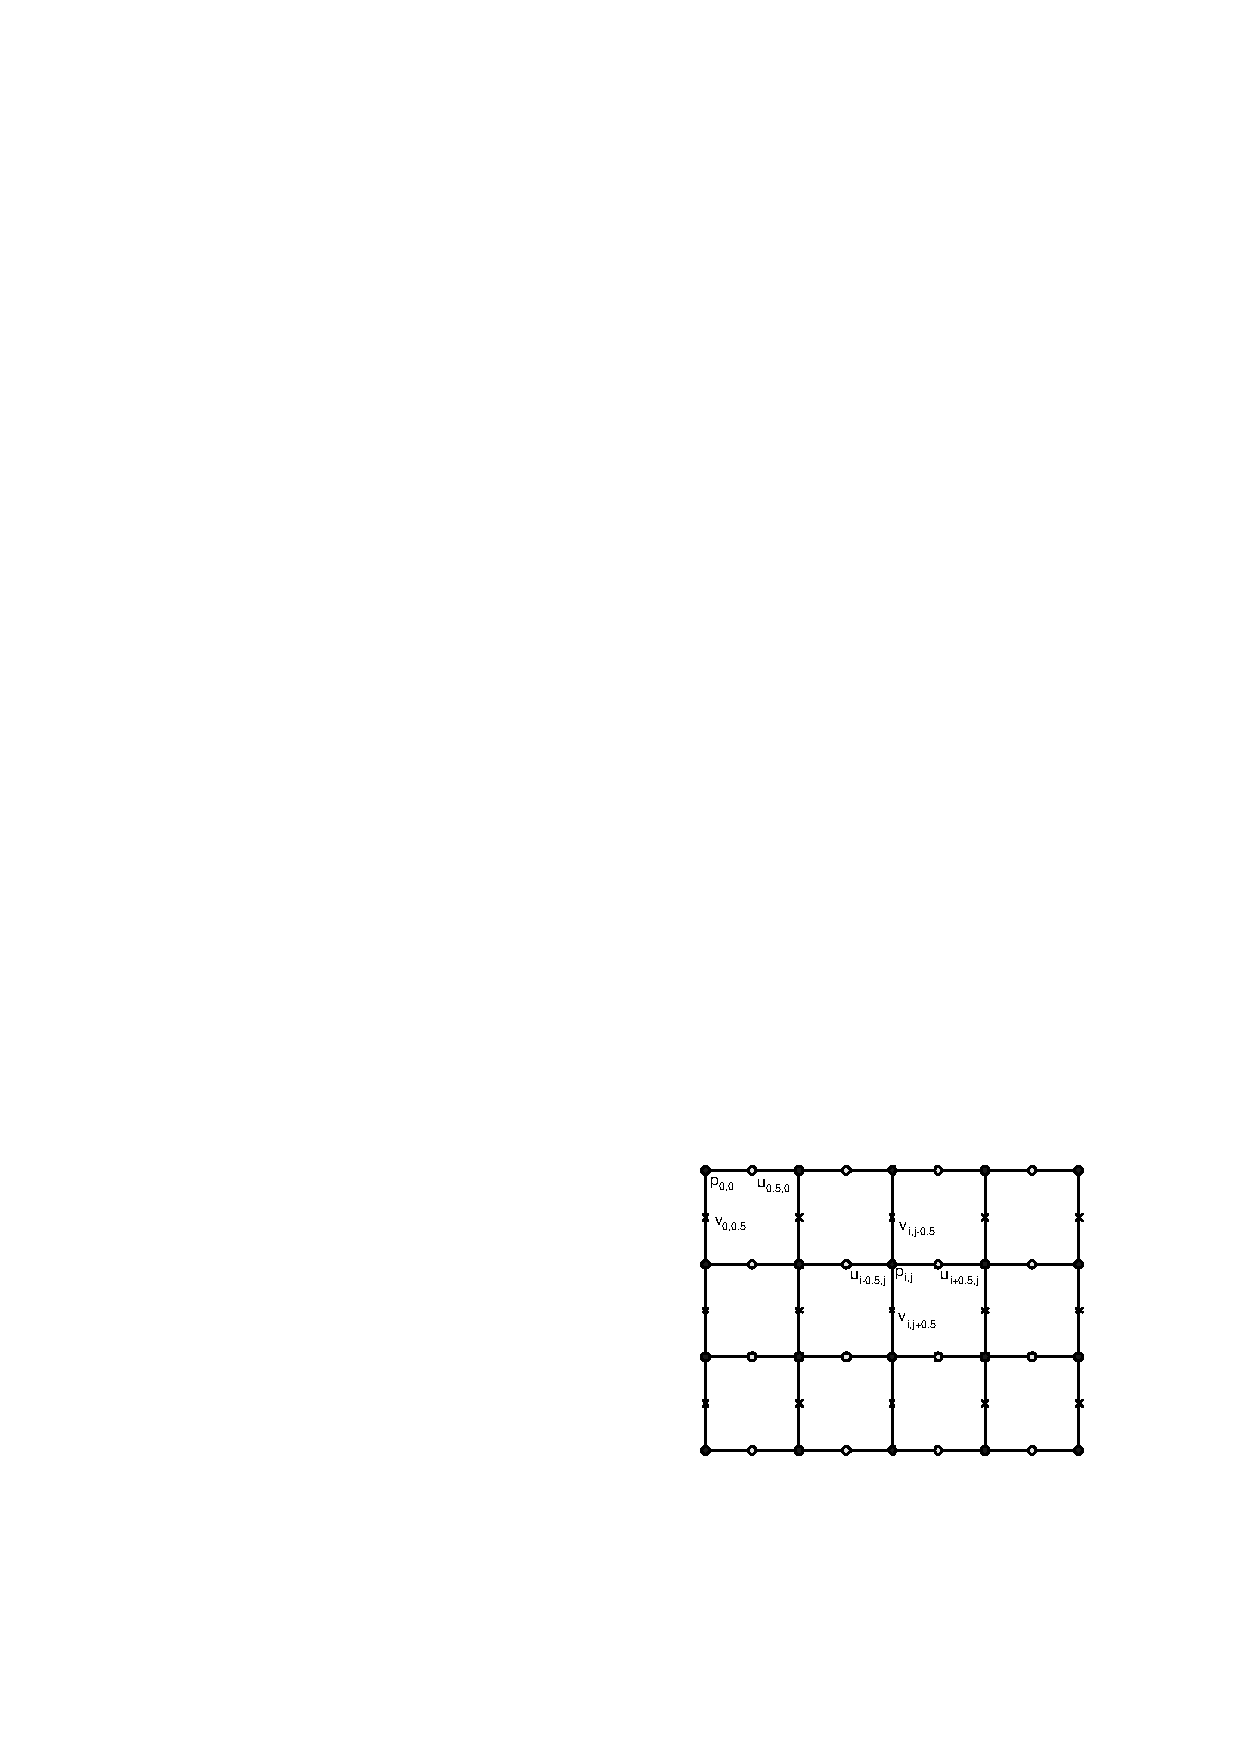
\includegraphics[width=0.4\textwidth]{./figures/StaggeredGrid.pdf}
\begin{tikzpicture}[ media/.style={font={\footnotesize\sffamily}},scale=1.75]

\draw[semithick,gray](-2,-1) grid (2,2);
\foreach \x in {-2,-1,...,2} {
      \foreach \y in {-1,...,2} {
              \draw[fill=blue!50] (\x,\y) circle(0.05);
       }
}

\foreach \x in {-1.5,-0.5,...,1.5} {
      \foreach \y in {-1,...,2} {
              \draw[red,ultra thick] (\x,\y) --++(45:0.05)  (\x,\y) --++(-45:0.05)  (\x,\y) --++(135:0.05)  (\x,\y) --++(-135:0.05);
       }
}

\foreach \x in {-2,-1,...,2} {
      \foreach \y in {-0.5,...,1.5} {
              \draw[ultra thick,green!40!black] (\x,\y) --++(0:0.05)  (\x,\y) --++(0:-0.05)  (\x,\y) --++(90:0.05)  (\x,\y) --++(-90:0.05);
       }
}

\node[below right,font=\footnotesize,blue] at (-2,2) {$p_{0,0}$};
\node[below right,font=\footnotesize,red] at (-1.5,2) {$u_{0.5,0}$};
\node[right,font=\footnotesize,green!40!black] at (-2,1.5) {$v_{0,0.5}$};

\node[below right,font=\footnotesize,blue] at (0,1) {$p_{i,j}$};
\node[below right,font=\footnotesize,red] at (-0.75,1) {$u_{i-0.5,j}$};
\node[right,font=\footnotesize,green!40!black] at (0,1.5){$v_{i,j+0.5}$};
\node[right,font=\footnotesize,green!40!black] at (0,0.5) {$v_{i,j+0.5}$};
\node[above,,font=\footnotesize,red] at (0.5,1) {$u_{i+0.5,j}$};
\end{tikzpicture}

\caption{\label{Stagger}交错网格}
\end{figure}

对于本文后面将要计算的一些算例, 由于固壁上的速度都为零, 所以本文将速度设置在边界上, 即水平速度设置在竖直边界上, 竖直速度设置在水平边界上. 考虑边界, 在物理边界外层设计半层虚拟网格. 比如在交错凹管道中的流动问题中, 其网格设置的示意图见图\ref{Stagger}
\begin{figure}[!htb]
\centering
%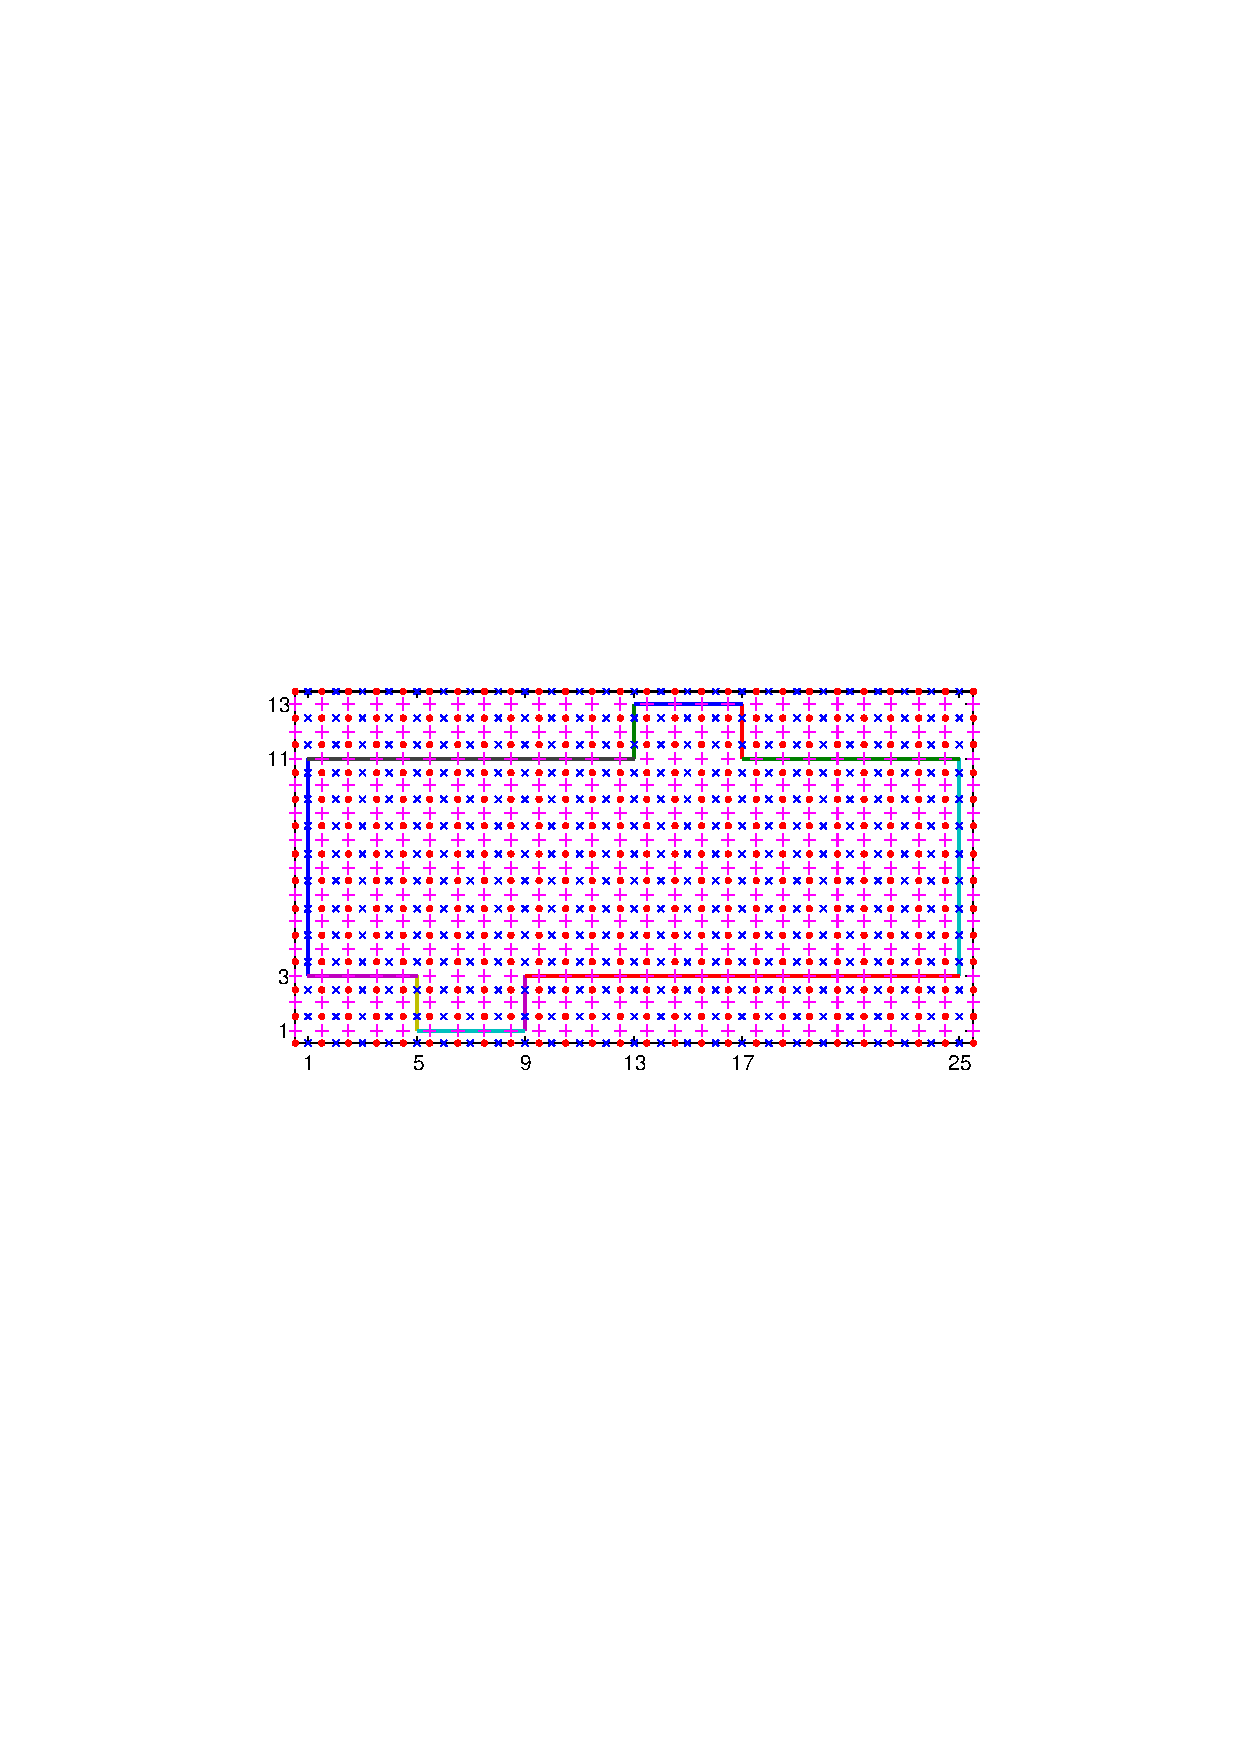
\includegraphics[width=0.7\textwidth]{./figures/mesh.pdf}
\begin{tikzpicture}[ media/.style={font={\footnotesize\sffamily}},scale=1.5]

%\draw[->,>=stealth',semithick,blue] (-0.25,0)node[left]{0.0}--(6.25,0) node[right]{$x$};

%\draw[->,>=stealth',semithick,blue] (0,-0.25)node[below]{$0.0$}--(0,3.25) node[above]{$y$};
\draw[step=0.25,gray,dotted,thin](-0.25,-0.25) grid(6.25,3.25);
%\draw[step=0.5,gray,thin](-0.25,-0.25) grid(6.25,3.25);
\draw[very thick](0,0.5)--(1,0.5)--(1,0)--(2,0)--(2,0.5)--(6,0.5);
\draw[very thick](6,2.5)--(4,2.5)--(4,2.5)--(4,3)--(3,3)--(3,2.5)--(3,2.5)--(0,2.5); 

\foreach \x in {-0.25,0.25,...,6.25} {
      \foreach \y in {-0.25,0.25,...,3.25} {
              \draw[fill=blue!50] (\x,\y) circle(0.05);
       }
}

\foreach \x in {-0.25,0.25,...,6.25} {
      \foreach \y in {0,0.5,...,3.25} {
              \draw[ultra thick,green!40!black] (\x,\y) --++(0:0.05)  (\x,\y) --++(0:-0.05)  (\x,\y) --++(90:0.05)  (\x,\y) --++(-90:0.05);
       }
}

\foreach \x in {0,0.5,...,6.25} {
      \foreach \y in {-0.25,0.25,...,3.25} {
              \draw[red,ultra thick] (\x,\y) --++(45:0.05)  (\x,\y) --++(-45:0.05)  (\x,\y) --++(135:0.05)  (\x,\y) --++(-135:0.05);
       }
}

\end{tikzpicture}

\caption{\label{Stagger}交错凹管道中的流动问题的网格设置:`.'表示压力$p$,`x'表示速度$u$,`+'表示速度$v$}
\end{figure}
从图\ref{Stagger}中可见, 在水平方向上速度$v$和压强$p$的节点数相等(本文设为$n_x+1$), 并且都比$u$多一个节点; 在竖直方向上, 速度$u$和压强$p$的节点数相等(本文设为$n_y+1$), 并且都比$v$多一个节点. 因此速度$u$, $v$及压强的节点数分别为
\[
n_x\times (n_y+1), \,\,\, (n_x+1)\times n_y, \,\,\, (n_x+1)\times(n_y+1)
\]
基于这种简单的交差网格的设置, 我们可以得到二阶精度的差分. 下面来讨论本文的差分格式.

\subsection{差分格式}
对于图\ref{steps}中的SIMPLE算法的步骤, 本文只需要对三个方程进行离散, 首先本文对动量方程式(\ref{momentumU})和式(\ref{momentumV})进行离散. 在动量方程的离散中, 各项的离散形式和精度见表\ref{Schemes}.
\begin{table}[!htb]
\centering
\caption{差分形式\label{Schemes}}
\begin{tabular}{|c|c|c|c|c|}
\hline
导数项 & 差分形式 & 导数项 & 差分形式 & 差分类型\tabularnewline
\hline
\hline
$u_{t}$ & $\frac{u^{n+1}-u^{n}}{\Delta t}$ & $v_{t}$ & $\frac{v^{n+1}-v^{n}}{\Delta t}$ & forward, $O(h)$\tabularnewline
\hline
$u_{x}$ & $\frac{u_{i+i,j}-u_{i-1,j}}{\Delta x}$ & $v_{y}$ & $\frac{v_{i+i,j}-v_{i-1,j}}{\Delta y}$ & central, $O(h^{2})$\tabularnewline
\hline
$u_{xx}$ & $\frac{u_{i+1,j}-2u_{i,j}+u_{i-1,j}}{(\Delta x)^{2}}$ & $v_{xx}$ & $\frac{v_{i+1,j}-2v_{i,j}+v_{i-1,j}}{(\Delta x)^{2}}$ & central, $O(h^{2})$\tabularnewline
\hline
$u_{yy}$ & $\frac{u_{i,j+1}-2u_{i,j}+u_{i,j-1}}{(\Delta y)^{2}}$ & $v_{yy}$ & $\frac{v_{i,j+1}-2v_{i,j}+v_{i,j-1}}{(\Delta y)^{2}}$ & central, $O(h^{2})$\tabularnewline
\hline
$(uu)_{x}$ & $u_{i,j}\frac{u_{i+1,j}-u_{i-1,j}}{2\Delta x}$ & $(vv)_{y}$ & $v_{i,j}\frac{v_{i+1,j}-v_{i-1,j}}{2\Delta y}$ & central, $O(h^{2})$\tabularnewline
\hline
$(uv)_{y}$ & $u_{i,j}\frac{v_{i+1,j}-v_{i-1,j}}{2\Delta y}+v_{ij}\frac{u_{i+1,j}-u_{i-1,j}}{2\Delta y}$ & $(uv)_{x}$ & $u_{i,j}\frac{v_{i+1,j}-v_{i-1,j}}{2\Delta x}+v_{ij}\frac{u_{i+1,j}-u_{i-1,j}}{2\Delta x}$ & central, $O(h^{2})$\tabularnewline
\hline
$p_{x}$ & $\frac{p_{i+1,j}-p_{i,j}}{\Delta x}$ & $p_{y}$ & $\frac{p_{i,j+1}-p_{i,j}}{\Delta y}$ & forward, $O(h)$\tabularnewline
\hline
\end{tabular}
\end{table}
动量方程式(\ref{momentumU})和式(\ref{momentumV})在图\ref{Stagger}所示的网格上的离散形式如下
\[
u_{i,j}^{n+1}=u_{i,j}^{n}+dt\Big[-A-B+\frac{1}{\mathrm{Re}}(C+D)-\frac{p_{i+1,j}-p_{i,j}}{\Delta x}\Big]
\]
\[
v_{i,j}^{n+1}=v_{i,j}^{n}+dt\Big[-E-F+\frac{1}{\mathrm{Re}}(G+H)-\frac{p_{i,j+1}-p_{i,j}}{\Delta y}\Big]
\]
其中
\begin{align*}
A & =u_{i,j}\frac{u_{i+1,j}-u_{i-1,j}}{2\Delta x}\\
B & =\frac{1}{4}\big(v_{i,j}+v_{i+1,j}+v_{i,j-1}+v_{i+1,j-1}\big)\frac{u_{i,j+1}-u_{i,j-1}}{2\Delta y}\\
C & =\frac{u_{i+1,j}-2u_{i,j}+u_{i-1,j}}{(\Delta x)^{2}}\\
D & =\frac{u_{i,j+1}-2u_{i,j}+u_{i,j-1}}{(\Delta y)^{2}}
\end{align*}
\begin{align*}
E & =v_{i,j}\frac{v_{i,j+1}-v_{i,j-1}}{2\Delta y}\\
F & =\frac{1}{4}\big(u_{i-1,j}+u_{i-1,j+1}+u_{i,j}+u_{i,j+1}\big)\frac{v_{i+1,j}-v_{i-1,j}}{2\Delta x}\\
G & =\frac{v_{i+1,j}-2v_{i,j}+v_{i-1,j}}{(\Delta x)^{2}}\\
H & =\frac{v_{i,j+1}-2v_{i,j}+v_{i,j-1}}{(\Delta y)^{2}}
\end{align*}

对于Poisson方程的求解, 本文利用四点迭代法求压力. 对于每一步Poisson方程的迭代, 其具体形式如下
\begin{equation}\label{Poisson}
p_{i,j}' = \frac{1}{a}\bigg[b\big(p_{i+1,j}'+p_{i-1,j}'\big)
+
c\big(p_{i,j+1}'+p_{i,j-1}'\big)+d\bigg]
\end{equation}
其中各项分别为下
\[
b= -\frac{\Delta t}{\Delta x^2},\: c = -\frac{\Delta t}{\Delta y^2},\: a = -2(a+b)
\]
对于式样(\ref{Poisson})的迭代方式非常简单. 每一步迭代, 本文都对每一个压强点用上式计算迭代后的值, 一步迭代完成后, 检查一下同一压强点上的迭代前后值相差的最大值是否为$\varepsilon=0$(实际计算过程中,$\varepsilon$取一个非常小的值, 当迭代前后的$p'$相差的最大值小于$\varepsilon$即认为迭代完成)
\subsection{边界条件}
在交错网格中, 边界处理相对于非交错网格较为复杂, 一些量的节点恰好在边界上, 而另一些节点则分布在边界两侧, 因此在施加边界条件时要非常小心, 本文对速度应用狄利克雷边界条件(Dirichlet boundary condition), 压强施加诺伊曼边界条件(Neumann boundary condition). 对于速度恰好在边界上的情况, 应用边界条件时真接将这些速度设为边界上的速度$U_b$(对于固壁边界条件, $U_b=0$), 比如在左右边界上的$u$及上下边界上的$v$. 而对于速度点分布在边界两边的情况, 比如在上下边界的$v$和左右边界的$v$, 其边界条件为
\[
\frac{u_{i,j}+u_{i,j+1}}{2} = U_b\, \Longleftarrow\, u_{i,j} = 2U_b - u_{i,j+1}\,\text{或}\, u_{i,j+1} = 2U_b - u_{i,j}
\]

对于边界上的压力的边界条件, 压力在边界法向上的导数$\partial p/\partial \mathrm{n}$由边界两边对应的两个压强点定义. 比如对于左边界, 诺伊曼边界条件为
\[
\frac{p_{i,j+1}-p_{i,j}}{dy} = 0 \, \Longrightarrow\, p_{i,j+1} = p_{i,j}
\]
实际上, 在本文的交错网格中, 固壁边界外的压力点并不参与到边界内速度的计算中, 因此在固壁上并不需要对压强施加边界条件. 只在最后结果的后处理中将压强平均到网格节点上时需要.


%\begin{figure}[!htb]
%\centering
%\animategraphics[poster = last, width = 0.7\textwidth, autoplay, controls, buttonsize=1em]{10}{./lax/}{0}{219}
%\caption{\label{laxanimate}采用Lax差分格式得到的密度$\rho$, 压强$p$, 速度$u$场}
%\end{figure}

\section{算例}
本文通过Fortran95编写了针对一般情况下不可压缩二维N-S方程的SIMPLE解法, 程序见附录. 只需在程序中给出相应的边界及边界条件(仅限于水平, 竖直, 及45度边界), 即可计算出相应的稳态结果. 用该程序很容易测试不同的情况. 应用该程序, 本文不仅测试了本次作业指定的交错凹管道中的流动问题, 还测试了不同是形状的通道, 以及通道中有不同形状和数量的障碍物的情况, 下面列举出部分本文测试的算例.
\subsection{交错凹管道中的流动问题}
交错凹管道中的流动问题是本次作业指定需要完成的题, 该问题初始设置如图\ref{case0}所示, 在一条高为2, 长为6的的通道中有两个凹槽. 管道的左端为初始入口, 入口处的水平速度$u$如图\ref{case0}中标注, $v=0$, $p=1$. 右端开口为出口边界条件.
\begin{figure}[!htb]
\centering
%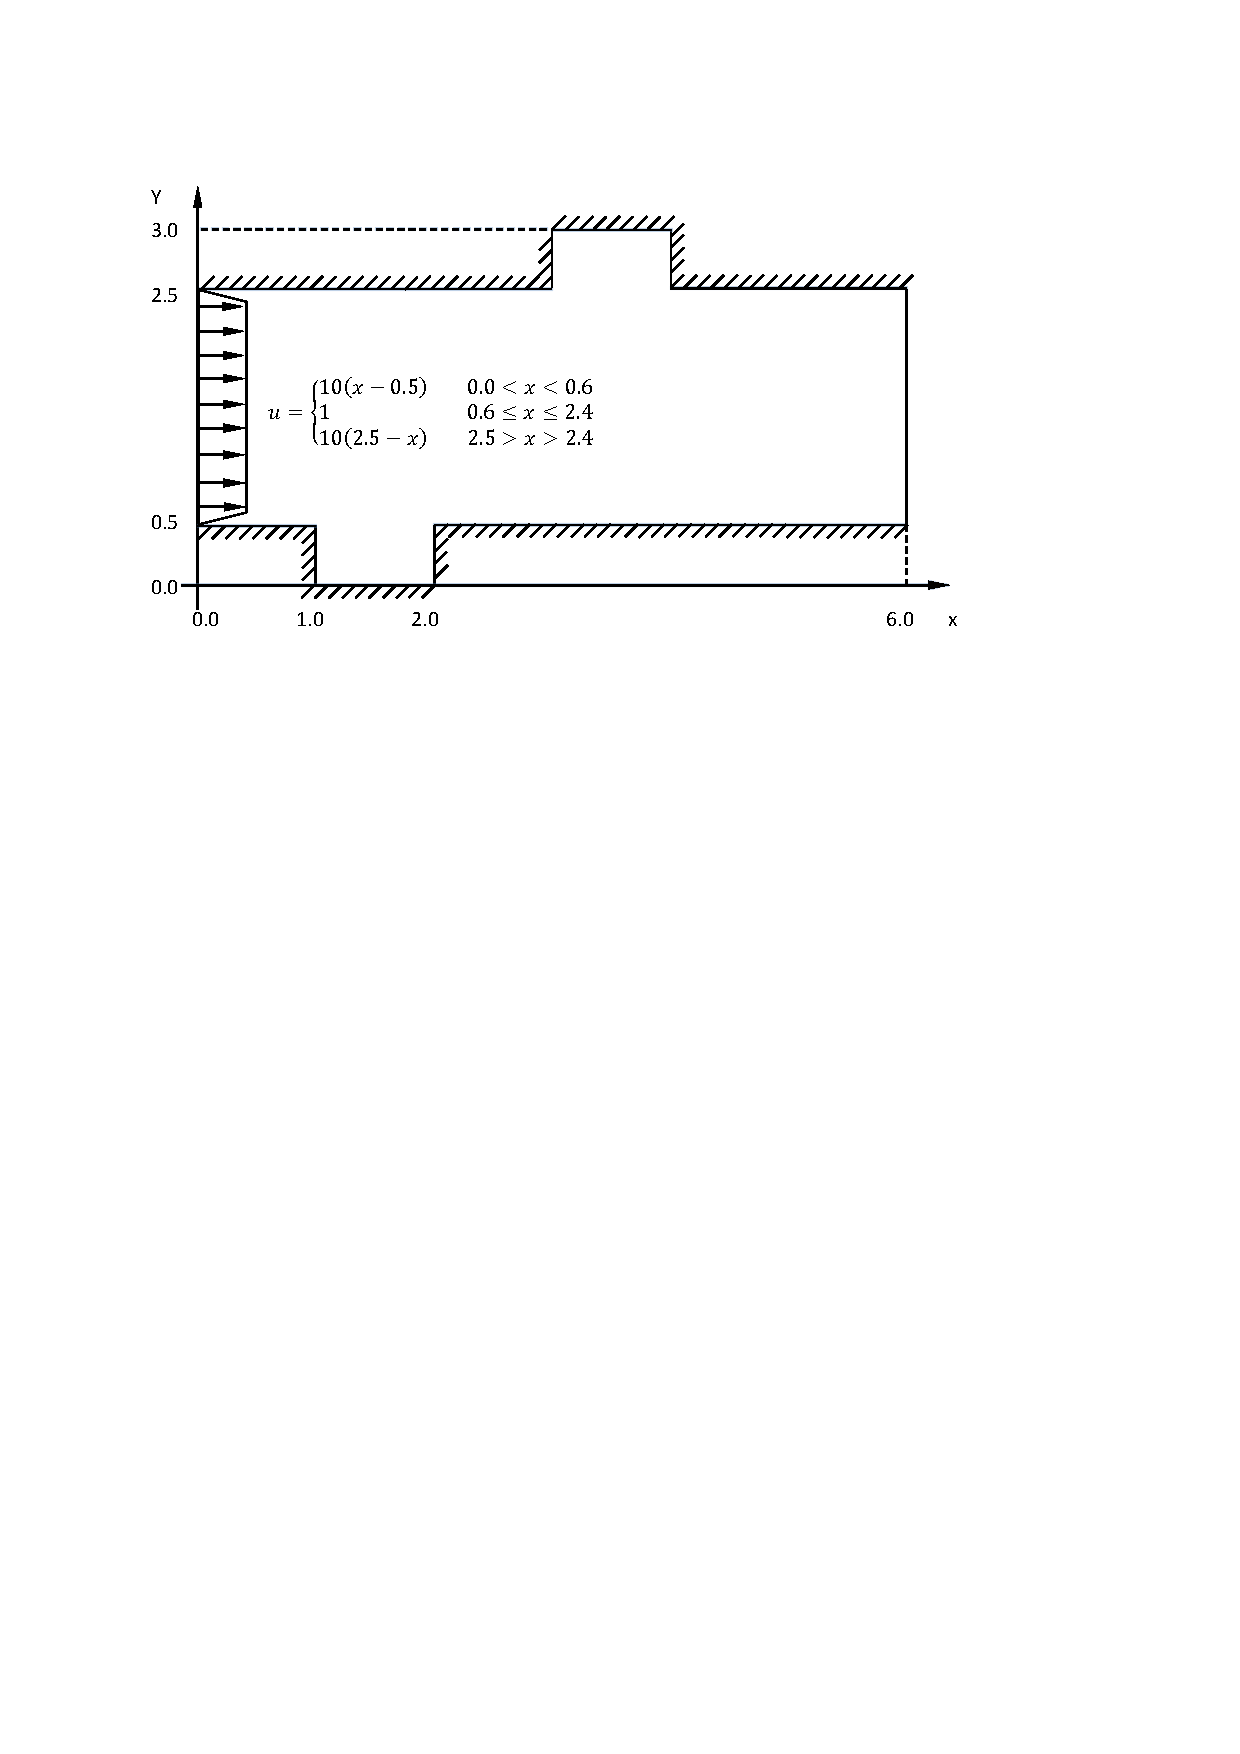
\includegraphics[width=0.8\textwidth]{./figures/case0.pdf}
\usetikzlibrary{%
    decorations.pathreplacing,%
    decorations.pathmorphing,arrows
}
\begin{tikzpicture}[ media/.style={font={\footnotesize\sffamily}},
    interface/.style={
        postaction={draw,decorate,decoration={border,angle=-45,
                    amplitude=0.3cm,segment length=2mm}}},scale=1.5]

\draw[->,>=stealth',semithick,blue] (-0.25,0)node[left]{0.0}--(6.25,0) node[right]{$x$};

\draw[->,>=stealth',semithick,blue] (0,-0.25)node[below]{$0.0$}--(0,3.25) node[above]{$y$};

\draw[semithick,interface](0,0.5)--(1,0.5); 
\draw[semithick,interface](1,0.5)--(1,0)--(2,0)--(2,0.5);
\draw[semithick,interface](2,0.5)--(6,0.5);

\draw[semithick,interface](3,2.5)--(0,2.5); 
\draw[semithick,interface](4,2.5)--(4,3)--(3,3)--(3,2.5);
\draw[semithick,interface](6,2.5)--(4,2.5);

\draw[semithick,densely dotted,blue](1,0)--(1,-0.25) node[below]{$1.0$} (2,0)--(2,-0.25) node[below]{$2.0$}
(3,2.5)--(3,-0.25) node[below]{$3.0$} (4,2.5)--(4,-0.25) node[below]{$4.0$} (6,0.5)--(6,-0.25) node[below]{$6.0$};

\draw[semithick,densely dotted,blue](0,0.5)--(-0.25,0.5)node[left]{0.5} (0,2.5)--(-0.25,2.5)node[left]{2.5} (3,3)--(-0.25,3)node[left]{3.0};

\draw[semithick,red,->,>=stealth'](0,0.75)--(0.6,0.75);
\draw[semithick,red,->,>=stealth'](0,1)--(0.6,1);
\draw[semithick,red,->,>=stealth'](0,1.25)--(0.6,1.25);
\draw[semithick,red,->,>=stealth'](0,1.5)--(0.6,1.5);
\draw[semithick,red,->,>=stealth'](0,1.75)--(0.6,1.75);
\draw[semithick,red,->,>=stealth'](0,2)--(0.6,2);
\draw[semithick,red,->,>=stealth'](0,2.25)--(0.6,2.25);
\draw[semithick,red](0,0.5)--(0.6,0.6)--(0.6,2.4)--(0,2.5);

\node[red,right] at (0.75,1.5) {
$u=\begin{cases}
10(x-0.5) & 0.0<x<0.6\\
1 & 0.6\leq x\leq2.4\\
10(2.5-x) & 2.4<x<2.5
\end{cases}$
};


\end{tikzpicture}

\caption{\label{case0}交错凹管道中的流动问题}
\end{figure}

\newpage
通过对图\ref{case0}所示的交错凹管道中的流动问题的SIMPLE计算, 本文得到了该问题的数值解, 即稳态的速度场和压力场. 图\ref{0u}和图\ref{0v}是计算得到的速度场. 从速度场可以看出, 在通道内近边界处的水平速度非常用小, 中间较大, 这说与无滑移边界条件完全符合. 另外在凹槽内, 水平速度非常用小.
\begin{figure}[!htb]
\centering
%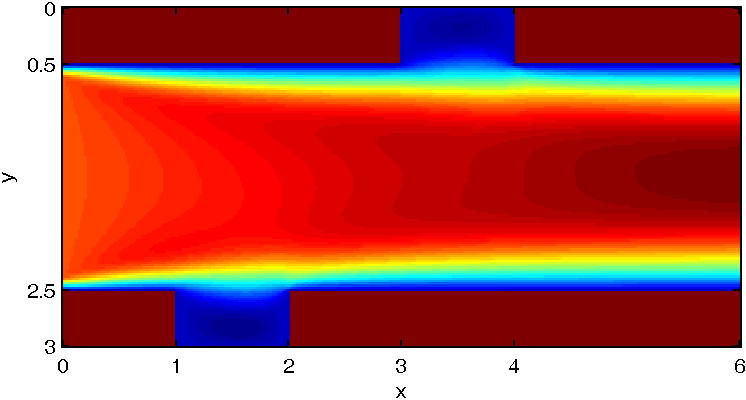
\includegraphics[width=0.6\textwidth]{./figures/00u.pdf}
\pgfplotsset{compat=1.7}
\begin{tikzpicture}
\begin{axis}[width=0.65\textwidth,height=0.325\textwidth,
xlabel={$x$},
%yticklabels={0.035,0.1,0.2,0.3,0.4,0.5},
ylabel={$y$},
xmin=0,xmax=6,ymin=0,ymax=3, 
yticklabel style={font=\scriptsize},
xticklabel style={font=\scriptsize},
xlabel style={font=\footnotesize},
ylabel style={font=\footnotesize},
legend style={font=\scriptsize,legend cell align=left},
]

\addplot graphics [xmin=0,xmax=6,ymin=0,ymax=3]{./figures/u0.pdf};
\end{axis}





\end{tikzpicture}

\caption{\label{0u}交错凹管道中的流动问题的$u$速度场}
\end{figure}
在角点处,速度$v$ 较大, 其它区域, 速度$v$几乎为零.
\begin{figure}[!htb]
\centering
%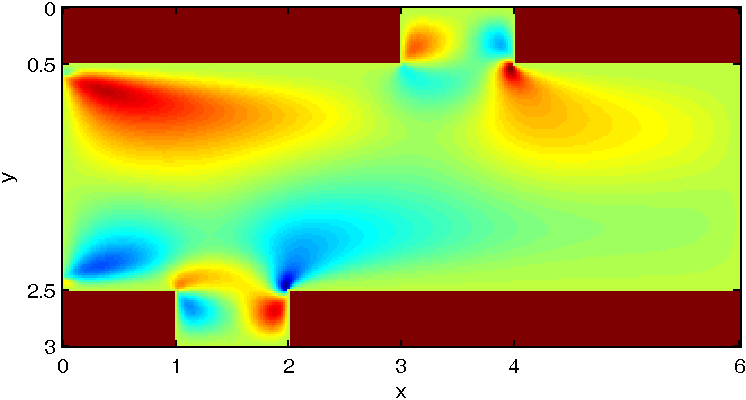
\includegraphics[width=0.6\textwidth]{./figures/00v.pdf}
\pgfplotsset{compat=1.7}
\begin{tikzpicture}
\begin{axis}[width=0.65\textwidth,height=0.325\textwidth,
xlabel={$x$},
%yticklabels={0.035,0.1,0.2,0.3,0.4,0.5},
ylabel={$y$},
xmin=0,xmax=6,ymin=0,ymax=3, 
yticklabel style={font=\scriptsize},
xticklabel style={font=\scriptsize},
xlabel style={font=\footnotesize},
ylabel style={font=\footnotesize},
legend style={font=\scriptsize,legend cell align=left},
]

\addplot graphics [xmin=0,xmax=6,ymin=0,ymax=3]{./figures/v0.pdf};
\end{axis}





\end{tikzpicture}

\caption{\label{0v}交错凹管道中的流动问题的$v$速度场}
\end{figure}
图\ref{0p}交错凹管道中的流动问题的压力场及流线图, 从该图中可以看出, 在两个凹槽内形成了两个涡, 中间流线基本场均水平, 在出口处, 流线完全水平, 压力均匀.
\begin{figure}[!htb]
\centering
%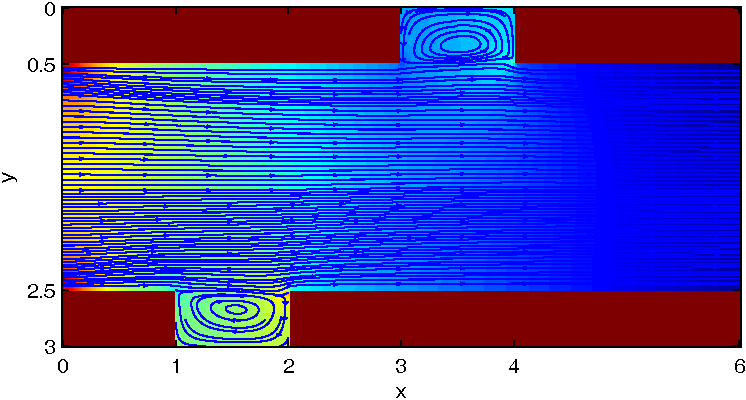
\includegraphics[width=0.6\textwidth]{./figures/00.pdf}
\pgfplotsset{compat=1.7}
\begin{tikzpicture}
\begin{axis}[width=0.65\textwidth,height=0.325\textwidth,
xlabel={$x$},
%yticklabels={0.035,0.1,0.2,0.3,0.4,0.5},
ylabel={$y$},
xmin=0,xmax=6,ymin=0,ymax=3, 
yticklabel style={font=\scriptsize},
xticklabel style={font=\scriptsize},
xlabel style={font=\footnotesize},
ylabel style={font=\footnotesize},
legend style={font=\scriptsize,legend cell align=left},
]

\addplot graphics [xmin=0,xmax=6,ymin=0,ymax=3]{./figures/p0.pdf};
\end{axis}





\end{tikzpicture}

\caption{\label{0p}交错凹管道中的流动问题的压力场及流线图}
\end{figure}


\subsection{其它算例}
交错凹管道中的流动问题外, 本文还对奇性方腔流, 弯折管道, 对称缩腰管道中的流动以及流场中有方块,三角等一个或多个障碍物的情况进行了测式.  下面给出了部分算例的测试结果.
\begin{figure}[!htb]
\centering
%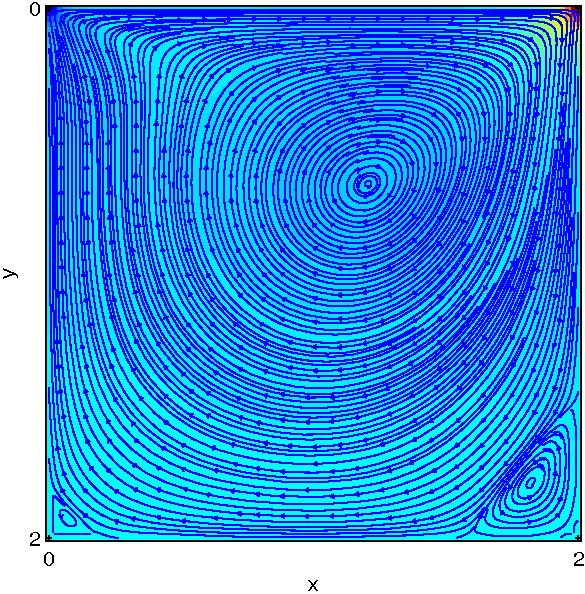
\includegraphics[width=0.6\textwidth]{./figures/04.pdf}
\pgfplotsset{compat=1.7}
\begin{tikzpicture}
\begin{axis}[width=0.65\textwidth,height=0.65\textwidth,
xlabel={$x$},
%yticklabels={0.035,0.1,0.2,0.3,0.4,0.5},
ylabel={$y$},
xmin=0,xmax=2,ymin=0,ymax=2, 
yticklabel style={font=\scriptsize},
xticklabel style={font=\scriptsize},
xlabel style={font=\footnotesize},
ylabel style={font=\footnotesize},
legend style={font=\scriptsize,legend cell align=left},
]

\addplot graphics [xmin=0,xmax=2,ymin=0,ymax=2]{./figures/p4.pdf};
\end{axis}





\end{tikzpicture}

\caption{奇性方腔流}
\end{figure}

\newpage

\begin{figure}[!htb]
\begin{minipage}[b]{.5\textwidth}
\centering
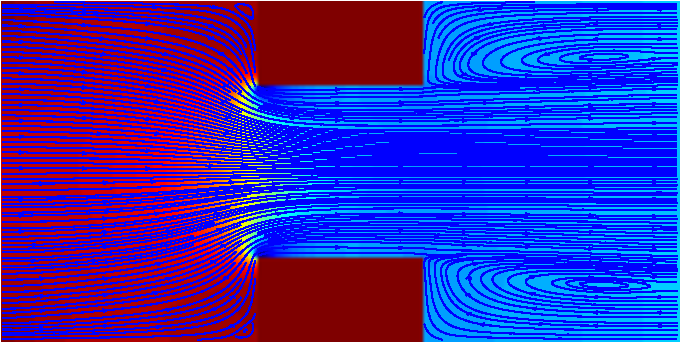
\includegraphics[width=0.95\textwidth]{./figures/05.pdf}
\caption{对称缩腰管道}
\end{minipage}
\begin{minipage}[b]{.5\textwidth}
\centering
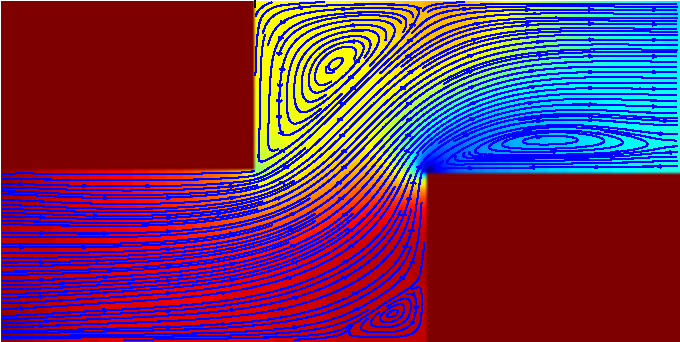
\includegraphics[width=0.95\textwidth]{./figures/06.pdf}
\caption{弯折管道}
\end{minipage}
\end{figure}

\begin{figure}[!htb]
\begin{minipage}[b]{.5\textwidth}
\centering
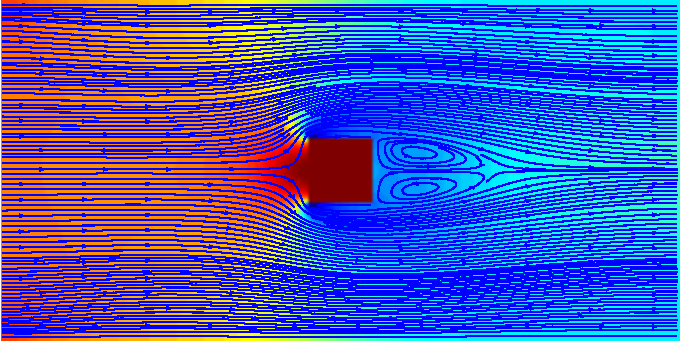
\includegraphics[width=0.95\textwidth]{./figures/01.pdf}
\caption{流场中一个方块情况}
\end{minipage}
\begin{minipage}[b]{.5\textwidth}
\centering
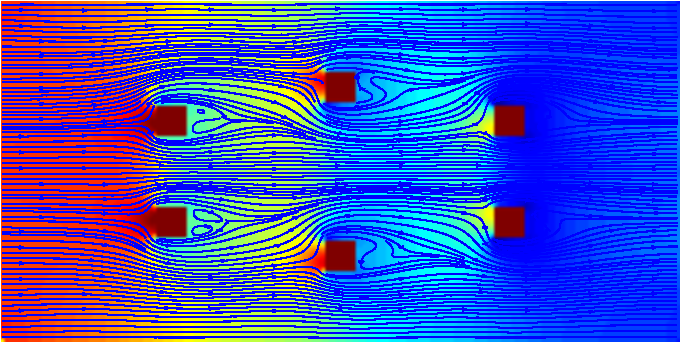
\includegraphics[width=0.95\textwidth]{./figures/03.pdf}
\caption{流场中多个方块情况}
\end{minipage}
\end{figure}

\begin{figure}[!htb]
\begin{minipage}[b]{.5\textwidth}
\centering
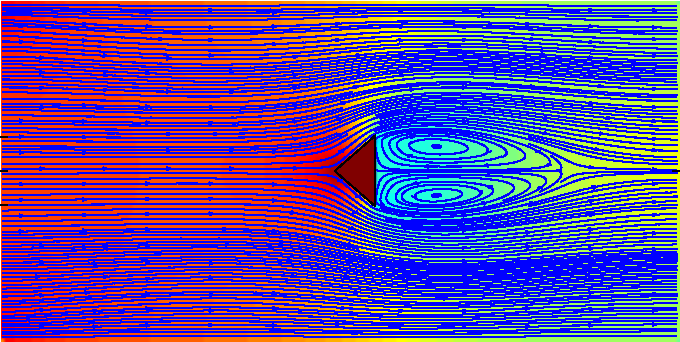
\includegraphics[width=0.95\textwidth]{./figures/02.pdf}
\caption{流场中三角形情况}
\end{minipage}
\begin{minipage}[b]{.5\textwidth}
\centering
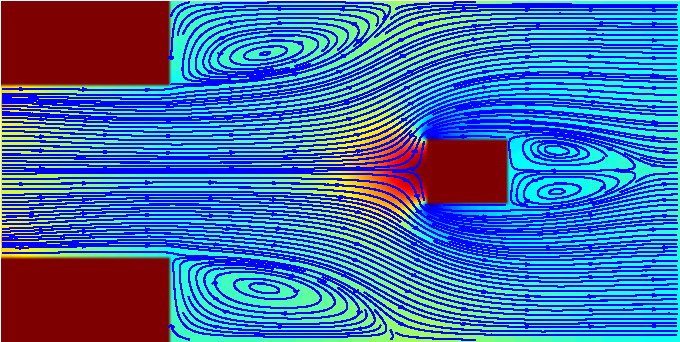
\includegraphics[width=0.95\textwidth]{./figures/07.pdf}
\caption{扩张流中方块情况}
\end{minipage}
\end{figure}

\begin{thebibliography}{99}
\bibitem{1} 张德良, 计算流体力学教程. 高等教育出版社. 北京, 2011.
\bibitem{2} Maciej Matyka. Solution to two-dimensional Incompressible Navier-Stokes Equations with SIMPLE, SIMPLER and Vorticity-Stream Function Approaches. Driven-Lid Cavity Problem: Solution and Visualization.
\bibitem{3} Benjamin Seibold. A compact and fast Matlab code solving the incompressible
Navier-Stokes equations on rectangular domains
\bibitem{4} SIMPLE algorithm. http://en.wikipedia.org/wiki/SIMPLE\_algorithm
\end{thebibliography}


\newpage
\appendix
\appendixpage
\begin{subappendices}
\section{CFD2dSimple.f90~~\attachfile{./codes/CFD2dSimple.f90}}
{\small
\fortranscript{./codes/CFD2dSimple}{}
}

\section{data2figure.m~~\attachfile{./codes/data2figure.m}}
{\small
\matlabscript{./codes/data2figure}{}
}
\end{subappendices}

\end{document} 
